%! Suppress = MissingImport
\section{Detailed Workflow}\label{sec:detailed-workflow}

This section is going to detail the new proposed workflow.
It's going through each step, by detailing exactly what have been changed,
modified or removed.

To keep this section straightforward and focused on the workflow, some
implementation details or advices will be omitted and moved to the next
sections of this chapter.

\subsection{Design \& Specs}\label{subsec:design-specs}
This first step of design and specifications is inherited from the
document-oriented approach of the waterfall methodology and V-model.
This step haven't really been improved nor modified and basically remains the
same.

The analysts will work with the stakeholders to understand their business
needs and formalize their requirements.
The architect will then design a solution that should be able to solve the
problem.
They will finally write the specifications of the solution that will fulfill
the global business needs.

This step is where the client is mostly involved during the workflow, because
once he validated the documentation, it should be a standalone source of
information for the whole development process.

% TODO populate requirements and solution specification in ALM tool
% TODO split into subsubsection if it's considered as too short

\subsection{Test Strategy}\label{subsec:test-strategy}
The test strategy step is also inherited from the traditional methodologies.
The manner or tool used to design a test strategy won't really be changed.
However, since the context in which the tests are going to be written and
executed will be different from the traditional one, we're going to mention
some important points.

\subsubsection{Previous context}
Before, in traditional methodologies, the test strategy simply consisted of
defining how to test each part of the specification, in an abstract way.
There were various information, such as the dataset or the account type to use
but the detailed steps weren't written yet.
It is a kind of feasibility study on how to test the application, to ensure
that every feature can be correctly tested.

When writing the test cases, the author can assume that when the test will
be executed, the implementation phase will be completed and therefore all the
features defined in the specification will be available.
The order of test writing wasn't a problem too, because the test will be
executed only once every tests will be written, so there's no need of
prioritization.

\subsubsection{New context}
In the new workflow, the context is different from the previous one.
Tests are not executed at the end anymore, but throughout the development
process.
Indeed, when a new test is written, it is intended to be used as an executable
specification and drive the implementation phase.
This will provide a quick feedback on the feature itself but also on the test
format.

At first glance, the ordering doesn't really matter since there should be
enough information regarding the scenario and the global documentation to
implement the feature.
Well in fact, the problem lies on the feedback duration.
Here is an example with a small set of modules and their dependencies.

\begin{figure}
    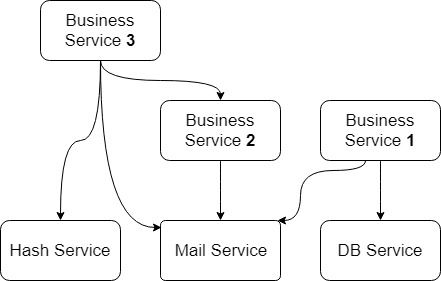
\includegraphics[width=\textwidth]{../../resources/images/solution/module_dependencies.png}
    \centering
    % TODO fix position with the related text
\end{figure}

In this figure, the \textit{Business Service 3} depends on 2 common modules
and 1 other business service.
When writing the scenarios, all the information will be available to the tester,
thanks to the comprehensive specification, so there won't be any problem when
writing it.

However, when the scenario will be submitted to the developers, they will
need all the dependent modules to be implemented in order to implement the
\textit{Business Service 3}.
If this scenario is written first, then it will take days to have the feedback.

Furthermore, they will have to work on modules that don't have their
scenarios written.
Which means that they either have to wait for them or start the
implementation without the tests, which would be like working the old
traditional way that we want to avoid.

\subsubsection{Defining the right strategy}
In order to reduce the feedback duration and let the tests drive the
implementation, the test strategy should not only cover how to test the
solution but also in which order they should be written.

The approach should be following the agile principle about building
progressively the application, step by step.
Every new test will produce a new feature or service and will add value
to the application.
The prioritization should be made regarding the importance of the module and
its dependencies, in order to have test that are easy to implement.

A feature that has a lot of unimplemented dependencies won't be a great
candidate at the beginning, because it will require too much effort to make
it pass.
These dependencies, usually common services, should therefore be tested
and implemented first, so they become available for other features.
The important idea here is to always try to produce a test, which is also an
executable specification, that is easily doable at the time it's released.

But there are some cases where it's okay to produce it even if it's not
quickly doable.
For example, when a module is implemented at 95\%, it's preferable to write
the last test, so the testers can complete this module and move to another one.
The developers will simply ignore this test for now and will take a look at
it when its dependencies will be correctly implemented.

The test strategy can also be discussed with the client.
This can be very useful during the prioritization,when defining the set of
core modules and services.
Both the client and analysts will share the same vision and understanding of
what's vital to the application and what is less important.

\subsection{Acceptance Test Kickoff}\label{subsec:acceptance-test-kickoff}
This new step occurs right after the validation of the test strategy.
Here, the team is going to set up the base of the acceptance tests that will
be used for the rest of the workflow.

In absolute, this step could have been omitted and its content included in
the test writing steps.
However, since the acceptance scenarios are going to be at the center of the
development process, they must be strong and reliable.
Therefore, they have a dedicated step to set up everything and validate the
scenario base before starting using it.

\subsubsection{Define the vocabulary}
The vocabulary used to write the scenarios is critical.
A scenario must be self explanatory, have clear intents by describing the
expected behaviour.
Hence it must use domain-specific words, so the analysts feel comfortable
when writing it and share the same words with the developers.

The definition of the vocabulary must not be done by only one side (analysts
or developers).
If so, the other team is likely to misunderstand the scenario or to miss the
important business aspect of a feature.
This would be just like in the traditional methods, where they were
interpreting and implementing a specification, without clearly understanding it.

Therefore during this step, at least the tech lead should be present with the
analysts, but it would be better to have several other members, such as the
architect or another developer.

The presence of the developers is very important because they will have to
implement the code of the scenarios.
Hence they can slightly adapt the vocabulary and the sentence format so it
will be easier to write and automate.

\subsubsection{Write the first scenarios}
Once the vocabulary is defined, the first scenarios can be written.
During the test strategy, the ordering have already been defined, so the
first scenarios to write are already known.
These scenario are going to be used as sample, to get familiarized
with vocabulary and adjust it if necessary.

During this phase, one important point to address is to define the correct
abstraction and granularity of the scenarios.
As said earlier, scenarios must be self explanatory and easily understood by
both the analyst and developer.

If the scenario is too abstract, then it will allow more interpretation and
the result is likely to diverge from the expected result of the writer.
In addition, it won't really \textit{drive} the implementation as it will be
too high level.

A contrario, a very detailed scenario will be less readable and will probably
lose its \textit{domain} aspect, as it's likely to simply specify the
technical requirements instead of describing a behavior.
A scenario too technical will also make the analysts less comfortable with, as
it won't use their domain words.

\subsubsection{Validate the base}
In order to validate the sample scenarios, the developers will write their
code and execute it with the analysts.

The first implementations will validate that the vocabulary used and the
scenario format is indeed executable and easily automated.
These implementation will be reused and extended throughout the development
process, so they must be validated as early as possible.

Once implemented, the scenario are going to be executed and validated using
some sort of shadowing.
Shadowing is a technique of knowledge transfer, where a new incomer will learn
how a person does its job, by observing him and doing the same thing and
eventually replacing him.
The previous person will validate the knowledge transfer by staying with the
new incomer but letting him actually do the job.

In our case, it won't really be shadowing, because the tests are not going to
learn from the testers.
However, when the tests will be executed, the testers will watch what they
are actually doing and see if the tests are valid and their verification
relevant.

This validation is a very important step to make the team confident regarding
their test implementations.
If these tests are correct, then the new tests produced using the same format
and vocabulary will also be reliable and trustful.

\subsection{Test Writing}\label{subsec:test-writing}
This step starts right after the acceptance test kickoff finishes and the
test base is validated.
The testers now have the tools to write the new tests, following what
has been defined in the test strategy.

\subsubsection{Continuous Backlog Filling}
This step runs in parallel of the implementation phase and is intended to
drive it by continuously fill the backlog of the dev team.
Having the two teams working parallel is a great thing as it will shorten the
global duration of the workflow.

In traditional methods, there was no problem since both team were working
with the specification and therefore could evolve independently.
However in this new workflow, the dev team advancement is now tied to the
advancement of the analysts as the scenarios drive the implementation.
This introduces new risks.

There are two different risks: starvation and long feedback duration. \\
Starvation will appear when the scenarios are produced at a lower rate than
they are consumed, that is the developers implement faster than the testers
write tests. \\
In the opposite case, when scenarios are created faster than they are
implemented, the feedback duration will increase as the developers won't
immediately work on the new scenarios.

\begin{figure}
    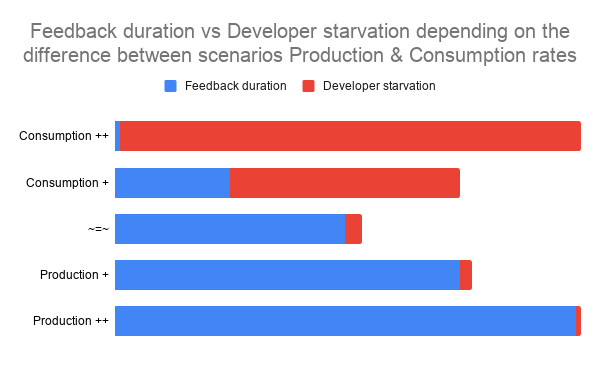
\includegraphics[width=\textwidth]{../../resources/images/solution/feedback_vs_starvation.png}
    \centering
\end{figure}

Developer starvation appears to be the worst risk, because it means
developers being paid for waiting the analysts to work.
A solution is to delay the start of the implementation phase and wait for a
certain amount of scenarios to be available.
But doing this will increase the feedback duration on the scenarios because
nobody will immediately work on the new scenarios.

There is no perfect formula and the scenarios production and consumption
rates aren't really predictable and can hardly be managed.
A balanced solution seems to trade a bit of feedback in order to reduce the
risk of developers starvation.
This is why the start of the implementation phase is slightly delayed in our
workflow.

\subsubsection{Continuous Extension}
When writing their scenarios, the analysts should try to reuse at most the
existing vocabulary and use the same scenario format.
However, as they are producing new scenarios for the rest of the
specification, they're likely to want to introduce new domain-specific words or
new kind of steps.

This extension of the domain vocabulary should be made with the tech lead and
some other developers, just like during the Acceptance Test Kickoff step.
As the scenario implementations are just normal code, they should therefore be
cleaned and refactored when possible.
These phases of domain extension are perfectly suited to do also some
refactoring, that is mainly removing the duplication.

Test refactoring is always a critical part, because it implies to modify the
only strong and reliable source of information of the application.
Verification post-refactor, such as the shadowing-like technique must be done
after to ensure that the scenario code base is still trustful.

\subsection{Implementation}\label{subsec:implementation}
The implementation step starts slightly after the test writing step, in order
to have a sufficient amount of scenarios to work with.
This phase will follow some principles and methods of Extreme Programming.

\subsubsection{Backlog consumption}
The backlog of scenarios is going to be the main source of tasks for the
developers.
The analysts will continuously add new scenarios throughout the
development process, which will drive the implementation phase.

When a scenario is consumed, it will be marked as Work In Progress (WIP).
This will allow to have a realtime overview of the features currently being
implemented.
We won't detail more the scenario lifecycle management as it will be detailed
in a further section.

\subsubsection{Work in pairs}
Most of the features will be implemented with Pair Programming.
As said in the state of the art, PP is useful to share practices and
knowledge across the team and catch small mistakes earlier by using two
brains instead of one.

It was also said that there was no perfect configuration and it varies a lot
across the project.
Sometimes, people really struggle to work in pairs and it becomes counter
productive to work that way.
Therefore, PP can be replaced by more frequent peer reviews.

\subsubsection{TDD in action}
For example, in the V-model, the implementation step was followed by two extra
steps: unit and integration phases.
These phases have been merged into this step, as we are going to work
in TDD\@.

The scenario are helpful to drive the implementation as BDD is an extension of
TDD\@.
However, the scenarios are not a replacement for the traditional unit and
integration tests.
Working with TDD implies to work and progress with very small (baby) steps.
A scenario step tends to be too high level and abstract to be the only tests.

Hence, when a scenario is assigned to a pair, the first thing to do is to
break the scenario in smaller features.
Pairing is especially helpful when breaking down features because it reduces
the risk of misunderstanding or missing an important business point.

Unit tests must be written to progressively build the feature bases.
Once it's done, the developers should move to integration test to add the new
features into the application.
The new integration tests should drive to the initial acceptance test.
The feature will be correctly implemented when the acceptance test will
pass.

\subsubsection{Feature Integration}
To integrate the code, a Continuous Integration platform should be available
to the team.
Build and test should continuously run, on every commit in order to detect as
soon as possible the common integration errors.

Popular git platform, like Github or Gitlab, offer great integration
mechanism like Merge Requests (MR).
Several validations can be added to a MR, such as triggering a build on the
remote CI platform, analyzing the code with a tool like Sonar or virtually
merge the code and build / analyze the merged branch.
Each feature should have its own MR in order to ensure that the future
codebase will stay as clean as it was before, without adding any regressions.

Merge Request should be created as soon as possible, that is when the
feature is assigned to a pair.
Even if the main point of MR is to validate the final implementation before
merging, it can also be useful throughout the implementation when the MR is
marked as \textit{Work In Progress (WIP)}.

A WIP tag simply indicates that the work is not ready to be integrated but
it doesn't mean that peer review can't be made.
Communication and feedback are at the core of this new workflow and this can
be applied to WIP MR\@.

WIP MR makes the current advancement available for everyone else in the
project, where each member can comment and propose new things.
This is especially handy when the team is not working with Pair Programming,
as it makes peer review easier.

\subsubsection{Feedback on the Scenario}
Eventually, when the feature is correctly implemented and integrated, the
developers may send some feedback regarding the scenarios.
Whether because the scenario was too abstract, too technical, missing a
business point etc.
This can only improve the quality of further scenarios.

\subsection{Qualification}\label{subsec:qualification}
The qualification step can start once both the test writing and
implementation finish.
At this point, all the scenarios are passed and all their Merge Requests have
been integrated.

At first glance, there is no need of this qualification step, since we
already have all our acceptance tests passing.
However, not everything can be automated or written as a scenario, like UI
style check.
Also, mistakes from either the analyst or the developer are still possible
and a last check can catch them before going to production.

\subsubsection{Last scenario shadowing}
The automated scenario should be validated a last time during this phase.
In absolute, every scenario should be run again with a tester that watches
the execution.
But since the scenarios share the same vocabulary and steps, only a subset of
scenarios can be validated.
This should be enough to trust the others.

\subsubsection{Manual tests}
During this phase, all the test cases that can't be automated are executed.
If possible, they should still be written in the scenario format, so it will
be easier to read and maintain.
However when a scenario is saying something like \textit{The UI should be good
looking and the buttons well displayed}, then the scenario format is not very
relevant.

There are also some cases where the test case is very complex and can hardly
be automated.
It's usually the case where a project will interact with a sphere of
projects, where some test cases will require a specific configuration or data
in the other projects.

\subsubsection{Defect lifecycle}
When a bug is detected during the qualification, a defect will be created.
This defect must contain a formalized sequence of steps to reproduce the bug,
a scenario if possible.
By adding a new scenario for each defect, we can ensure that these bugs will
immediately be detected if they reappear again.
